%%%%%% Compile using latex, then dvips, then ps2pdf %%%%%%%%%%%%%

\documentclass{beamer}

%\documentclass[handout]{beamer}

%\includeonlyframes{current}

\mode<presentation>
{
%  \usetheme{Warsaw}
%  \usetheme{Frankfurt}
%  \usetheme{Singapore}
\usetheme{Boadilla}
}

\usepackage{times}
\usepackage[T1]{fontenc}
\usepackage[english]{babel}
\usepackage[latin1]{inputenc}

\usepackage{tikz}
\usepackage{pgflibraryshapes}
\usetikzlibrary{shapes}

\usepackage{graphics}
%\usepackage[draft]{graphics}

\usepackage{color}
\usepackage{xspace}
\usepackage{amsmath}
\usepackage{bm}
\usepackage{pgfpages}
\usepackage{fancybox}
\usepackage{threeparttable}
\usepackage{bbding}
\usepackage{booktabs}
\usepackage{fancyvrb}

\setbeamersize{text margin left=0.5cm,text margin right=0.5cm}

\setbeamercolor{equation.box}{fg=blue,bg=yellow!50!white}
\setbeamercolor{postit}{fg=black,bg=yellow!75!white}


%\graphicspath{{D:/teaching/figs/}}

%Additional commands

\DefineVerbatimEnvironment{ColorVerbatim}{Verbatim}%
  {formatcom=\color{black},commandchars=\\\{\}}

% Abbreviations for equations and lists

\newenvironment{shitemize}{
\begin{itemize}
\setlength{\parskip}{0pt} \setlength{\itemsep}{10pt}
\setlength{\parsep}{0pt}
%\setlength{\baselineskip}{7mm}
\setlength{\baselineskip}{8mm} }{\end{itemize}}

\newcommand{\bi}{\begin{itemize}}
\newcommand{\ei}{\end{itemize}}
\newcommand{\I}{\item}

% for a bulleted list nested within another bulleted list
\newcommand{\nestedbi}{\begin{itemize}}
\newcommand{\nestedei}{\end{itemize}}

% for a bulleted list with larger spacing between lines
\newcommand{\bibig}{\begin{itemize}}
\newcommand{\eibig}{\end{itemize}}

\newenvironment{senumerate}{\begin{enumerate}
\setlength{\parskip}{0pt} \setlength{\itemsep}{3pt}
\setlength{\parsep}{0pt} \setlength{\baselineskip}{10mm}
}{\end{enumerate}}


\newenvironment{shenumerate}{\begin{enumerate}
\setlength{\parskip}{0pt}
\setlength{\itemsep}{2pt}
\setlength{\parsep}{0pt}
}{\end{enumerate}}

\newcommand{\beq}{\begin{equation}}
\newcommand{\eeq}{\end{equation}}

\newcommand{\bea}{\begin{eqnarray}}
\newcommand{\eea}{\end{eqnarray}}

\newcommand{\beas}{\begin{eqnarray*}}
\newcommand{\eeas}{\end{eqnarray*}}

\newcommand{\ben}{\begin{enumerate}}
\newcommand{\een}{\end{enumerate}}

\newcommand{\beqs}{\begin{eqnarray*}}
\newcommand{\eeqs}{\end{eqnarray*}}



% for a section heading
\newcommand{\sect}[1]{
     {\large{\bf #1}}\vspace{0.05in}}

% for a subsection heading
\newcommand{\subsect}[1]{{\bf #1}\vspace{0.05in}}

% for a subsubsection heading
\newcommand{\subsubsect}[1]{{\it{#1}}\vspace{0.05in}}

% Misc.
\newcommand{\etal}{{\it et al.}}
\newcommand{\winbugs}{{\sc WinBUGS }}

% spaces
\newcommand{\negsp}{\vspace{-0.5cm}}
\newcommand{\possp}{\vspace{0.5cm}}

% Maths
%\usepackage{D:/teaching/maths}     % my maths style file

\newcommand{\EE}{\mathrm{I\!E}}  %% Expectation
\newcommand{\VV}{\mathrm{Var}} %% Variance

\newcommand{\bbeta}{\boldsymbol{\beta}}
\newcommand{\btheta}{\boldsymbol{\theta}}
\newcommand{\bnu}{\boldsymbol{\nu}}
\newcommand{\pmat}{\boldsymbol{p}}
\newcommand{\bx}{\boldsymbol{x}}

\newcommand{\pr}{\ensuremath{\mathbb{P}}}

\newcommand{\sis}{{\sigma^2}}

\newcommand{\E}{\mathbb{E}}

\newcommand{\No}{\text{Normal}}
\newcommand{\Ga}{\text{Gamma}}
\newcommand{\Uni}{\text{Uniform}}
\newcommand{\Bin}{\text{Binomial}}

\newcommand{\pari}{\hspace{\parindent}}

\title[Introduction to Bayesian Analysis (MSc)]
{\Huge{Lecture 9 \vspace{5mm}\\Further hierarchical models}}
\author[Further Hierarchical Models]
{}

\institute[Lecture 9]
{}
\date[]
{}


\begin{document}

\begin{frame}[t]
  \titlepage
\end{frame}

\begin{frame}
\frametitle{Outline}
There is huge scope for elaborating the basic hierarchical models
discussed in the previous lecture to reflect additional structure and complexity
in the data, e.g.\vspace{0.5mm}
\bi
\I Adding covariates at different levels of the hierarchy\vspace{0.5mm}
\I Adding further levels to
   the hierarchy (patients within wards within hospitals,
   pupils within schools within local authorities, $\ldots$)\vspace{0.5mm}
%\I Adding non-nested (cross-classified) levels (patients within
%GPs crossed with hospitals, $\ldots$)\vspace{0.5mm}
\I Repeated observations on
   some/all units (longitudinal data)\vspace{0.5mm}
 \I Modelling temporal or spatial structure
in data, $\ldots$\vspace{1mm}
\ei
In this lecture, we will discuss:\vspace{0.5mm}
\bi
\I Hierarchical models for count data and including covariates\vspace{0.5mm}
\I Hierarchical models for longitudinal data\vspace{0.5mm}
%\I Cross-classified models
\ei
\end{frame}

\begin{frame}
\frametitle{Hierarchical models for count data: Disease mapping}
\bibig
\I In disease mapping, we are interested in modelling counts of disease cases
   collected on each of a number of geographical areas within a study
   region\vspace{1mm}
\I Here we consider data on the observed number of cases of childhood leukaemia, $y_i$, diagnosed in a 10 year period
   in each of $i=1,\ldots,879$ areas (electoral wards) in London (data from Thames Cancer Registry)\vspace{1mm}
\I Using national age/sex-standardised reference rates for leukaemia and Census population counts, we can also calculate the
    expected number of cases, $E_i$, in each area\vspace{1mm}
\I Assume a Poisson likelihood for the disease count in each area:
   $$y_i \sim \hbox{Poisson}(\mu_i); \;\;\;\; \mu_i = \lambda_i E_i; \;\;\;\; i=1,\ldots,879$$
\I We have 879 {\it distinct} relative risk parameters
$\lambda_i$\vspace{1mm}
\I What prior should we specify for each $\lambda_i$?
\eibig
\end{frame}

\begin{frame}
\frametitle{Different modelling assumptions}
\vspace{2mm}{\bf Identical parameters}\\\vspace{2mm}
Assume $\lambda_i = \lambda \;\;\;\; \hbox{for all}\; i$ and assign a prior
   $$ \lambda \sim \hbox{Gamma}(a, b)$$
   with \alert{\it {specified values}} of $a$ and $b$, e.g.
      $$ \lambda \sim \hbox{Gamma}(1, 1)$$
      \vspace{-6mm}
   \bi
   \I[$\rightarrow$] conjugate Poisson-gamma model
   \ei
\vspace{3mm}
{\bf Independent parameters}\\\vspace{2mm}
Assume independent vague priors for each relative risk, e.g.
   $$\lambda_i \sim \hbox{Gamma}(0.1, 0.1), \;\;\;\;\; i=1,\ldots,879$$
\bi
      \vspace{-6mm}
\I[$\rightarrow$] This will give estimates of the posterior mean for $\lambda_i  \approx
y_i/E_i$, which is the MLE (also termed standardised morbidity ratio, SMR)
\ei
\end{frame}

\begin{frame}
\frametitle{Different modelling assumptions (continued)}
{\bf Similar (exchangeable) parameters}\\ \vspace{2mm}
Specify a \alert{hierarchical} random effects prior:
   $$\lambda_i \sim \hbox{Gamma}(a, b), \;\;\;\;\; i=1,\ldots,879$$
   where $a$ and $b$ are \alert{{\it unknown parameters}} to also be \alert{estimated}\vspace{2mm}
   \bi
\I[$\rightarrow$] assign hyperprior distributions to $a$ and $b$\vspace{2mm}
\I[$\rightarrow$] what is a suitable hyperprior for these parameters?
\ei
\end{frame}

\begin{frame}
\frametitle{A more flexible hierarchical prior for the relative risks}
\bibig
\I A gamma random effects prior for the $\lambda_i$ is mathematically convenient,
but may be restrictive:\vspace{1mm}
  \nestedbi
  \I covariate adjustment (regression) is difficult\vspace{1mm}
  \I no possibility for allowing spatial correlation between
     risks in nearby areas\vspace{2mm}
  \nestedei
\I A normal random effects prior for $\log \lambda_i$ is more flexible:
\beqs
y_i & \sim & \hbox{Poisson}(\mu_i= \lambda_i E_i ) \\[2pt]
\log \lambda_i & = & \alpha + \theta_i \\[2pt]
\theta_i & \sim & \hbox{Normal}(0, \sis)
\eeqs
\I Need to specify hyperprior distributions for\vspace{1mm}
     \nestedbi
     \I[] $\sis$ (between-area variance), e.g.~$\sigma^{-2} \sim \hbox{Gamma}(0.001, 0.001)$ \vspace{1mm}
     \I[] $\alpha$ (mean log relative risk), e.g.~$\alpha \sim \hbox{Normal}(0, 10000)$
     \nestedei
\eibig
\end{frame}

\begin{frame}
\frametitle{Parameter Interpretation}
\bibig
\I $\theta_i$ are the \alert{random effects}\vspace{2mm}
\I $\lambda_i = \exp(\alpha + \theta_i) =$ relative risk in area
   $i$ compared to expected risk based on age and sex of population\vspace{2mm}
\I $\theta_i$ can also be thought of as a latent variable which
   captures the effects of unknown or unmeasured area level
   covariates\vspace{2mm}
\I If these area level covariates are spatially structured
   (e.g.~environmental effects), our model for $\theta_i$
   should allow for this (i.e.~replace normal random effects
   distribution by spatial distribution --- not covered in this course)\vspace{2mm}
\I The variance of the random effects ($\sigma^2$) reflects
   the amount of extra-Poisson variation in the data
\eibig
\end{frame}

\begin{frame}
\frametitle{Ranking in hierarchical models}
\bi
\I Recent trend in UK towards ranking \lq institutional' performance e.g.~schools,
   hospitals or areas\vspace{1mm}
\I Rank of a point estimate is a highly unreliable summary statistic\vspace{0.5mm}
  \bi
  \I would like measure of uncertainty about rank\vspace{1mm}
  \ei
\I Bayesian methods provide posterior interval estimates for ranks\vspace{1mm}
\I For the leukemia example, at each MCMC iteration, ranking sampled values of
$\lambda_1,\ldots,\lambda_{879}$  gives sample from posterior distribution of ranks for each area\vspace{1mm}
\I See Goldstein and Spiegelhalter (1996) for further discussion on ranking\vspace{1mm}
\ei
BUGS contains \lq built-in' options for ranks:\vspace{0.5mm}
\bi
\I {\tt Rank} option of {\tt Inference} menu monitors the rank of the elements of a specified
vector\vspace{0.5mm}
\I {\tt rank(x[],i)} returns the rank of the ith element of {\tt x}\vspace{0.5mm}
\I {\tt ranked(x[],i)} returns the value of the ith-ranked element of {\tt x}
\ei
\end{frame}

\begin{frame}
\frametitle{Quantile ratios to summarise level 2 variability}
\bi
\I Unclear how to define or calculate the VPC for generalised linear hierarchical models\vspace{1mm}
\I Alternative summary of variability between units in a hierarchical
model is to rank the random effects and calculate the difference or ratio between two
units at opposite extremes\vspace{1mm}
\I For the leukemia example, suppose we consider the 5$^{th}$ and 95$^{th}$ percentiles
of the area relative risk distribution\vspace{0.5mm}
\bi
\I  let $\lambda_{5\%}$ denote the relative risk of leukemia for the area ranked
at the 5$^{th}$ percentile\vspace{0.5mm}
\I  let $\lambda_{95\%}$ denote the relative risk of leukemia for the area ranked
at the 95$^{th}$ percentile\vspace{0.5mm}
\I then QR$_{90} = \frac{\lambda_{95\%}}{\lambda_{5\%}} = $ ratio of relative risks of leukemia between the top
and bottom 5\% of areas\vspace{1mm}
\ei
\I Using MCMC, we can calculate the ranks, and hence the QR$_{90}$, at each
iteration, and hence obtain a posterior distribution for QR$_{90}$
\ei
\end{frame}

\begin{frame}[fragile]
{\it BUGS code}
\begin{footnotesize}
\begin{verbatim}
model {
 for(i in 1 : N) {
  Y[i] ~ dpois(mu[i])
  log(mu[i]) <- log(E[i]) + alpha + theta[i]
  theta[i] ~ dnorm(0, tau) # area random effects
  lambda[i] <- exp(alpha + theta[i]) # area relative risk
 }
 # Priors:
 alpha ~ dnorm(0, 0.0001) # vague prior on overall intercept
 tau ~ dgamma(0.5, 0.0005) # precision of area random effects
 sigma <- 1/sqrt(tau)      # between-area sd of random effects

 # 90% quantile ratio for area relative risks
 QR90 <- ranked(lambda[],835)/ranked(lambda[],44)

 #rank
 for(i in 1 : N) {
  rank.lambda[i] <- rank(lambda[], i) # rank of area i
 }
}
\end{verbatim}
\end{footnotesize}
\end{frame}

\begin{frame}
\frametitle{Results for childhood leukaemia example}
Parameters of interest:\vspace{2mm}
\bibig
\I $e^{\alpha+\theta_i}$ ({\tt lambda[i]}) = relative risk of leukaemia in area $i$
relative to expected (see map)\vspace{2mm}
\I $\sigma$ ({\tt sigma}) = between-area standard deviation of log relative risk of leukaemia\vspace{1mm}
   \bi
  \I posterior mean and 95\% interval = 0.46 (0.34, 0.62)\vspace{2mm}
    \ei
\I QR$_{90}$ ({\tt QR90}) = 4.7 (95\% interval 2.9 to 7.5)\vspace{1mm}
  \bi
  \I so 4.7-fold variation in relative risk
      of leukemia between top and bottom 5\% of areas
  \ei
\eibig
\end{frame}

\begin{frame}
\frametitle{Maps of estimated area-specific RR of leukaemia}
\centerline{\scalebox{0.5}{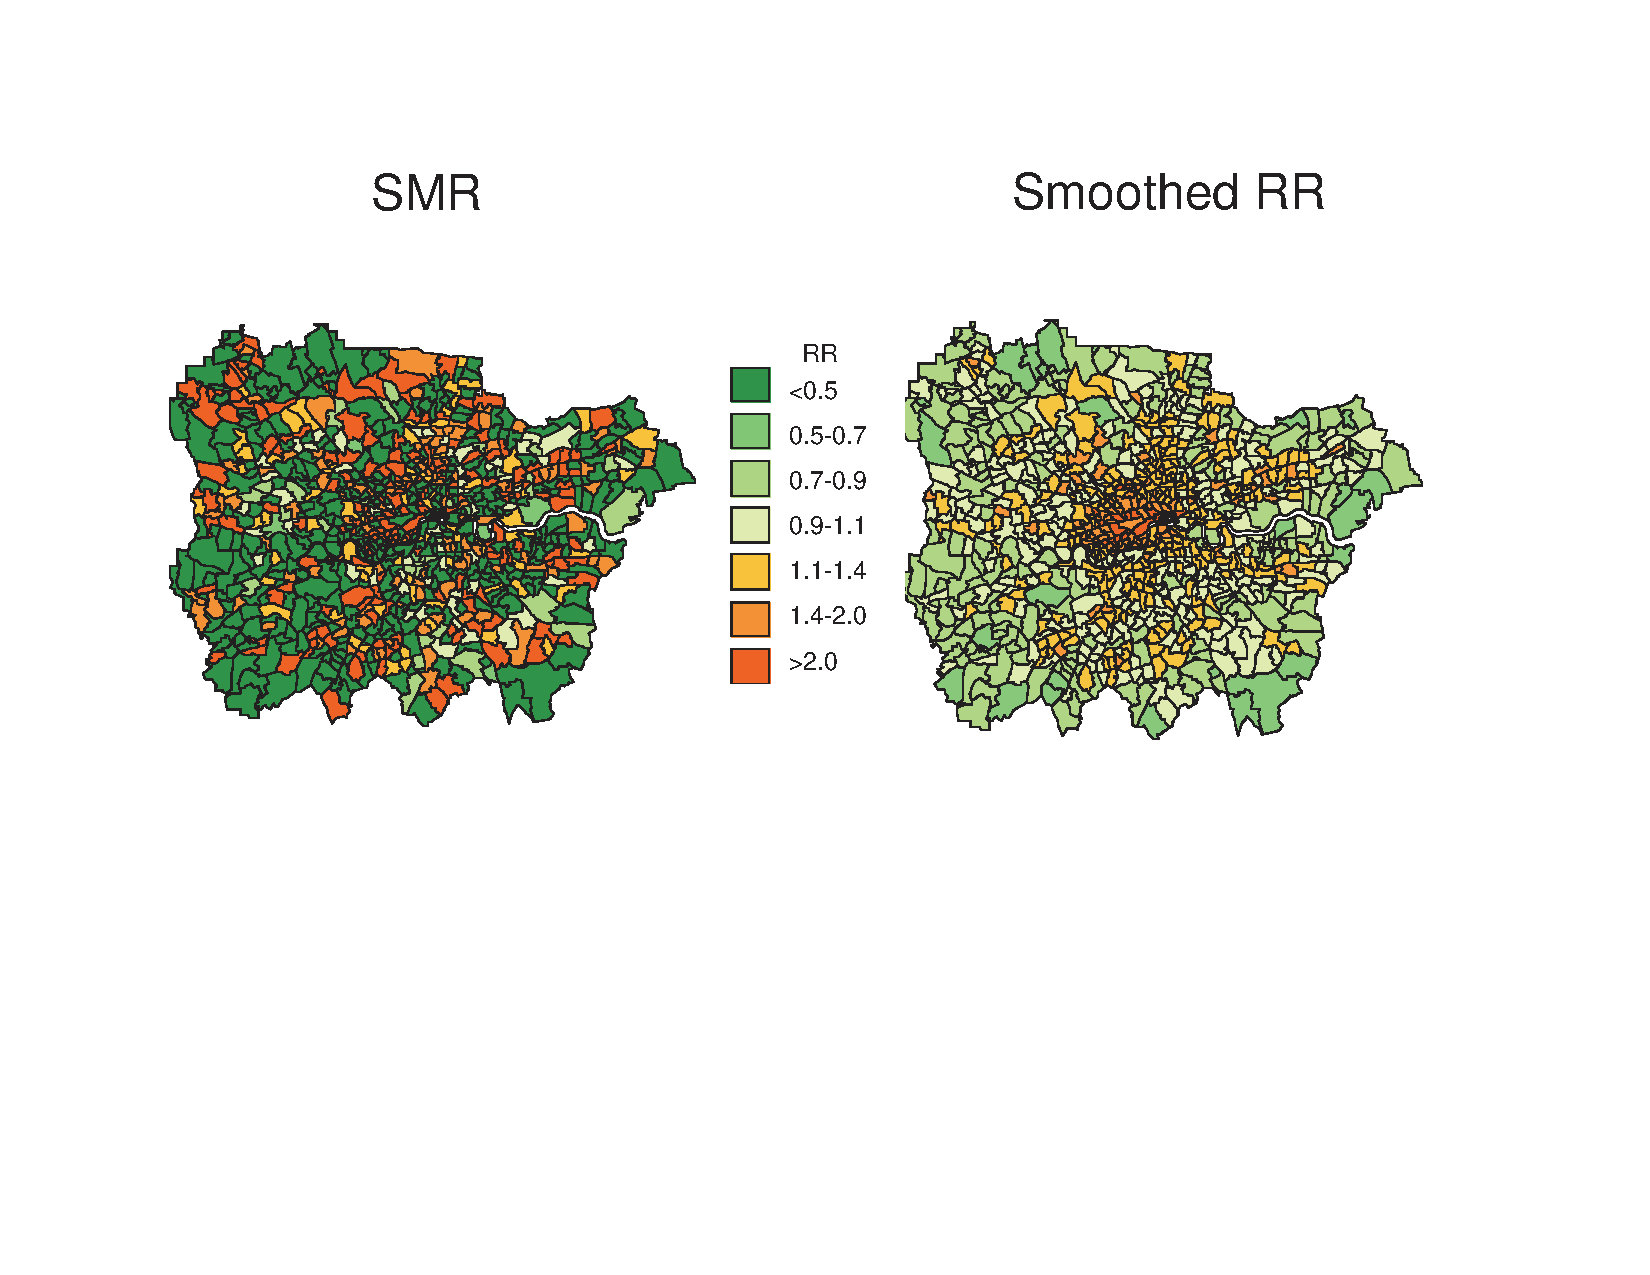
\includegraphics{figures/leuk-maps-smoothed}}}
\end{frame}

\begin{frame}
\frametitle{SMR versus posterior mean RR for selected areas}
\vspace{-12mm}
\centerline{\rotatebox{90}{\scalebox{0.9}{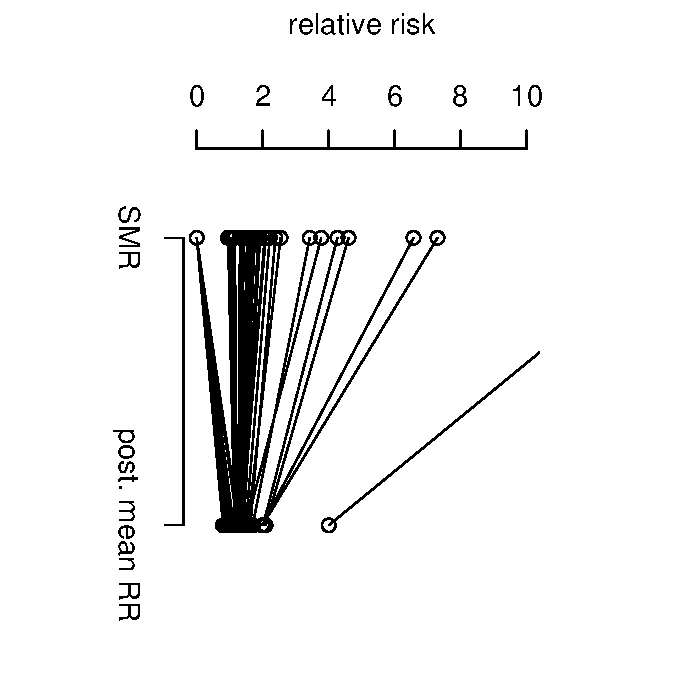
\includegraphics{figures/shrinkage}}}}
\end{frame}

\begin{frame}
\frametitle{Point estimate and 95\% interval for relative risk in selected
areas}
\centerline{\scalebox{0.6}{\includegraphics{figures/SMR-vs-posteriorRR}}}
\end{frame}

\begin{frame}
\frametitle{Posterior distribution of area ranks}
\centerline{\scalebox{0.45}{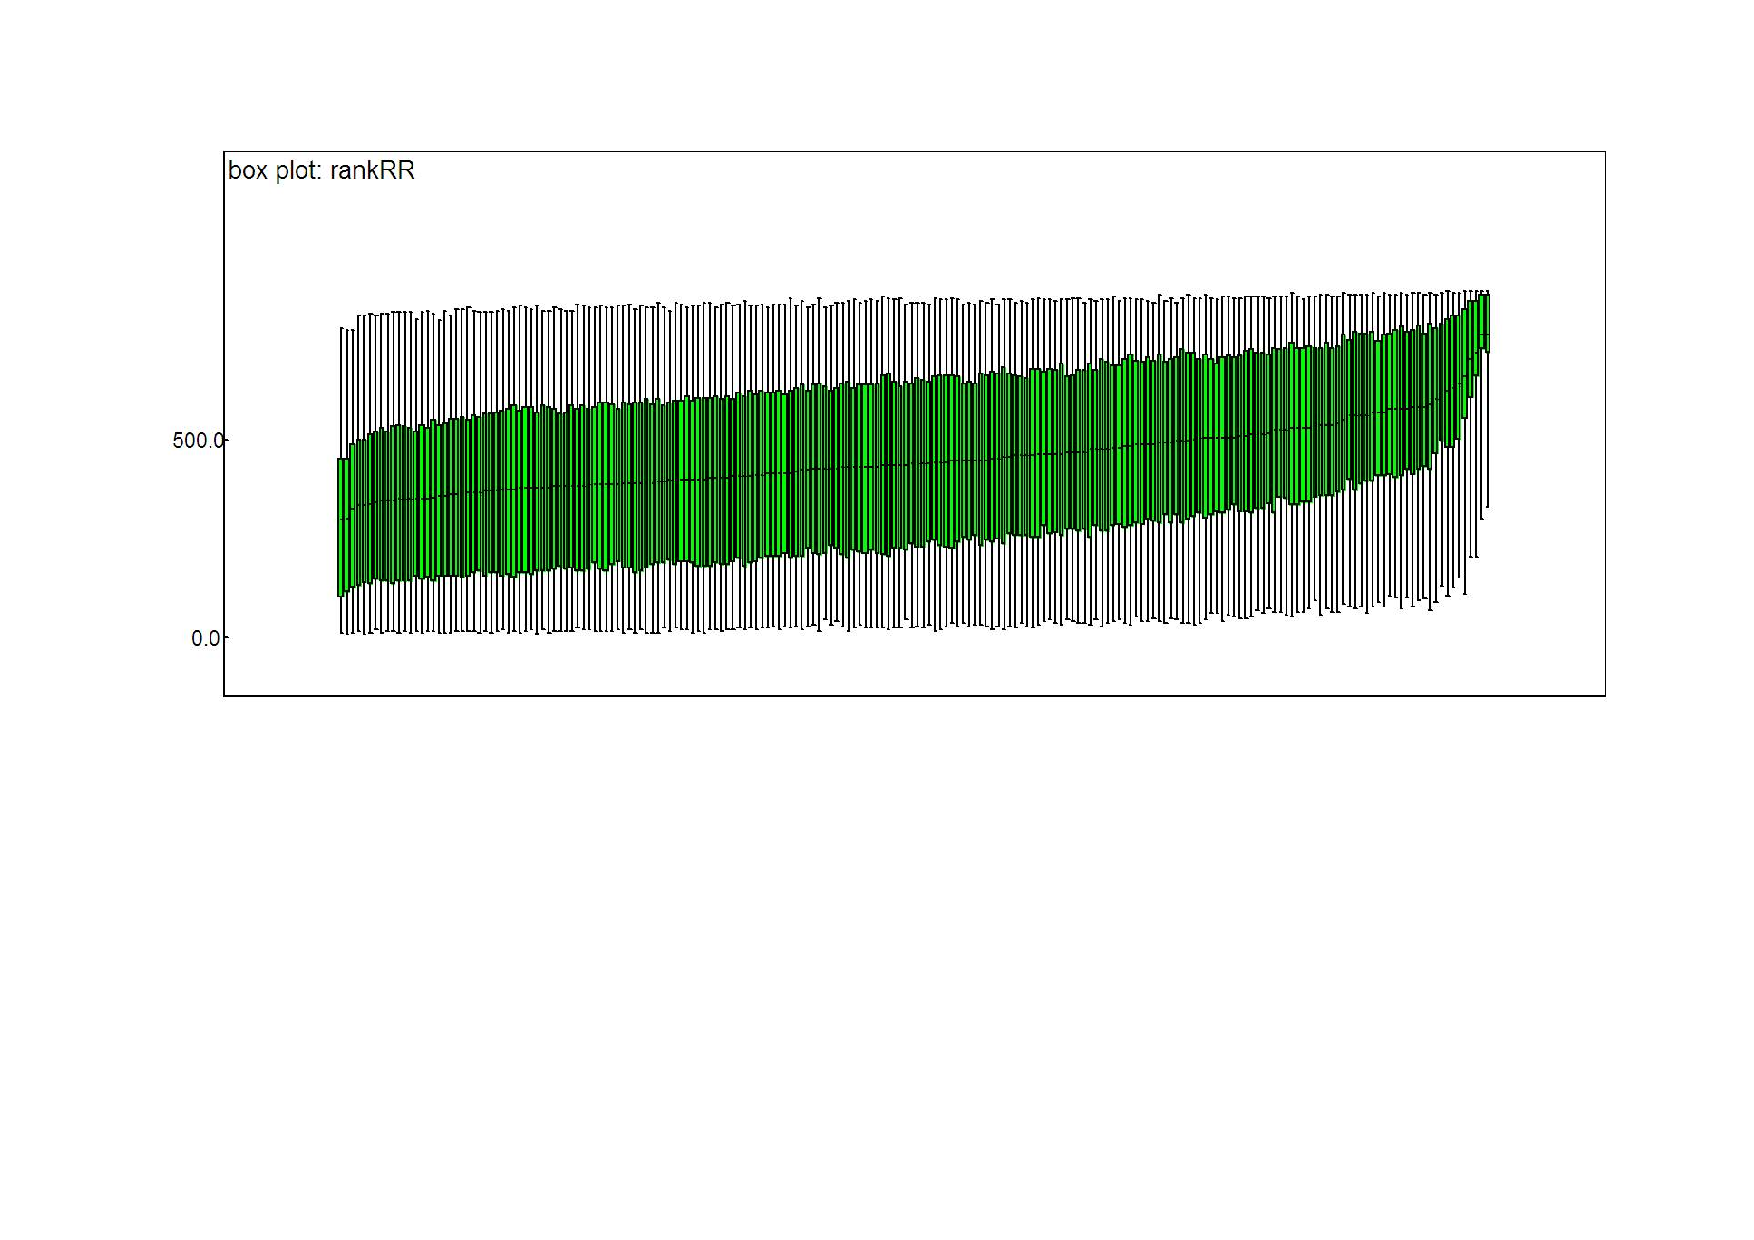
\includegraphics{figures/leuk-ranks}}}
\end{frame}

\begin{frame}
\frametitle{Including covariates in hierarchical models}
\vspace{-12mm}
\hspace{-15mm}\scalebox{0.45}{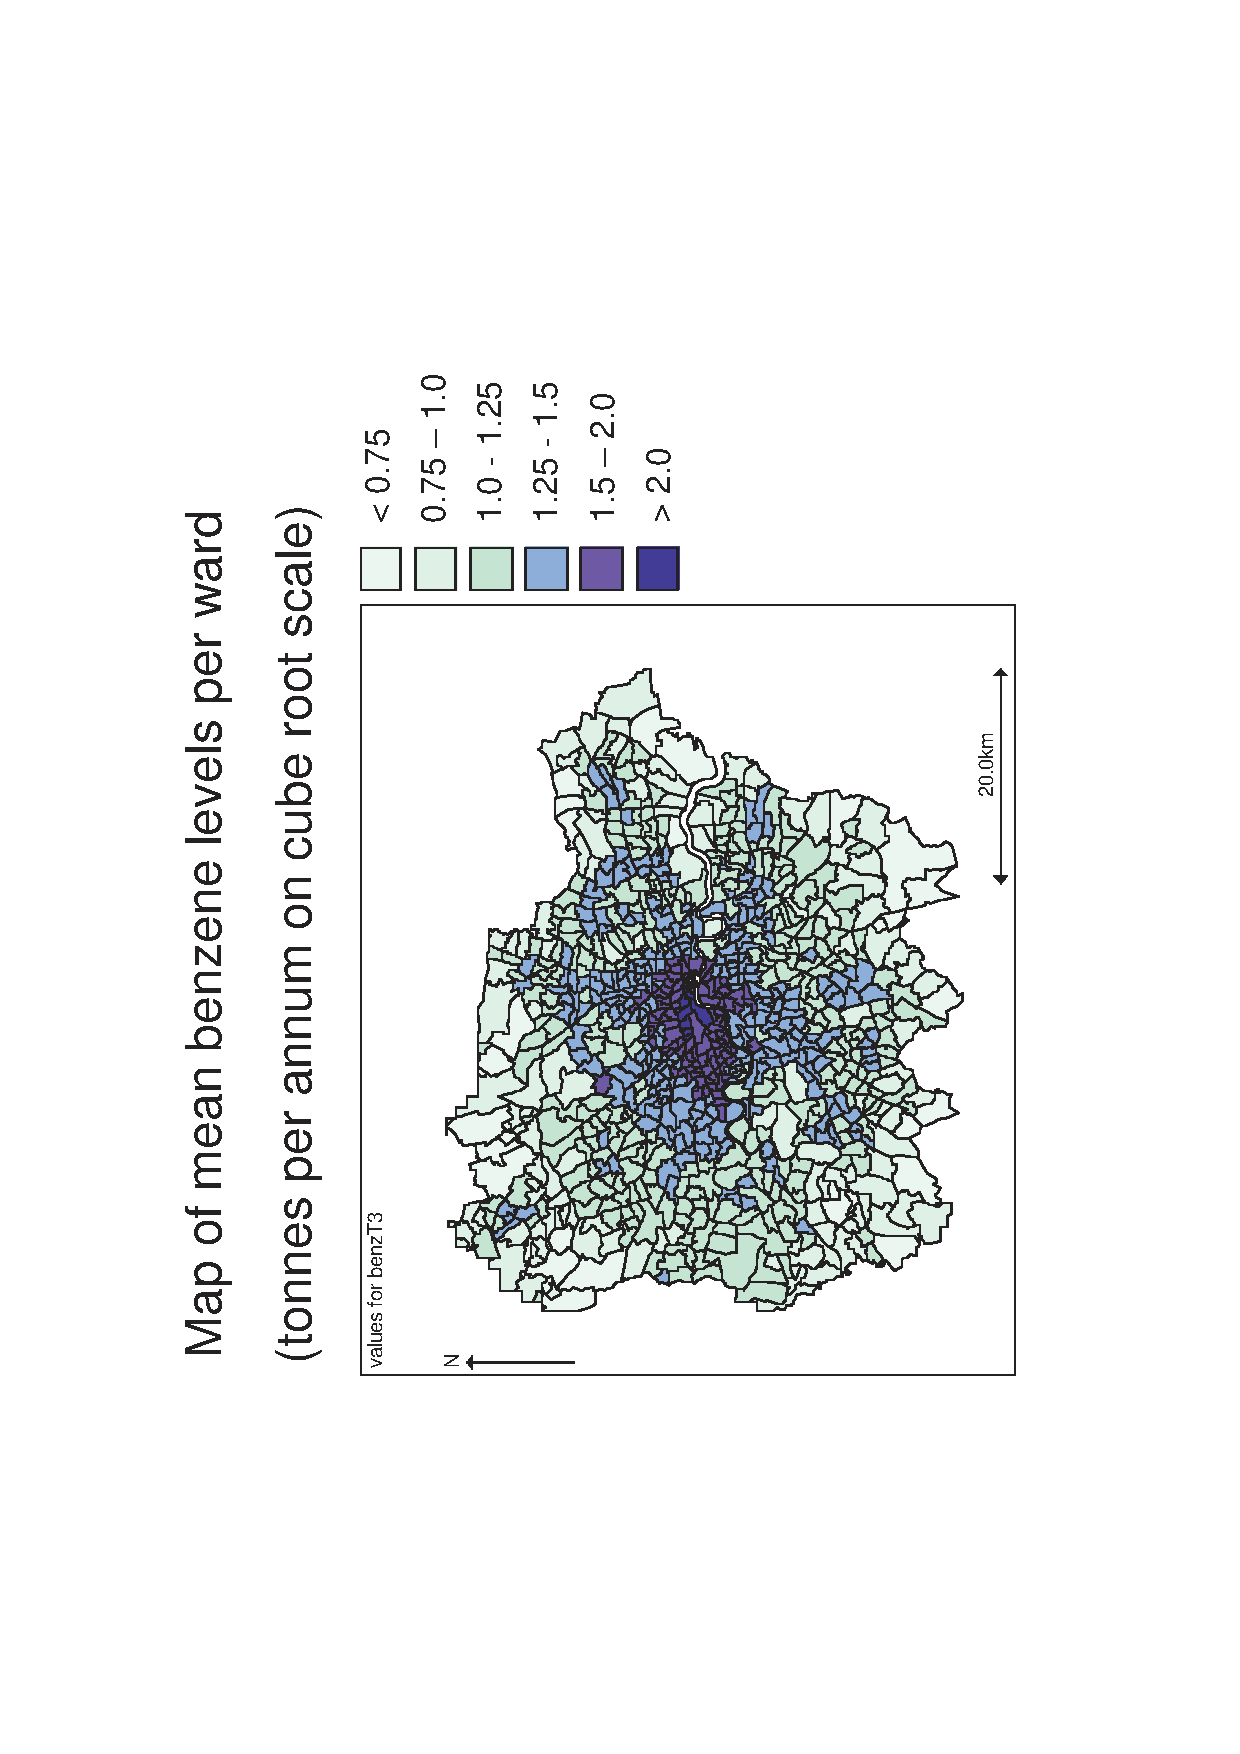
\includegraphics{figures/leuk-maps-benz}}
\vspace{-15mm}
\bibig
\I Can we explain some of the variation in risk of leukaemia by environmental exposure to benzene?
\eibig
\end{frame}

\begin{frame}
\frametitle{Including covariates in hierarchical models}
\bi
\I Let $X_i$ = average benzene emissions (tonnes per annum) in ward $i$\vspace{2mm}
\I Include $X$ as a covariate in the hierarchical model:
\ei\vspace{-2mm}
\begin{eqnarray*}
y_i & \sim & \hbox{Poisson}(E_i \lambda_i); \;\;\; i=1,\ldots,873 \\[3pt]
\log \lambda_i & = & \alpha + \beta X_i + \theta_i\\[3pt]
\theta_i  &\sim&  \hbox{Normal}(0, \sigma^2)\\[3pt]
\alpha, \beta, \sigma^2 & \sim & \hbox{vague priors}
\end{eqnarray*}
\end{frame}

\begin{frame}[fragile]
{\it Extract from BUGS code}
\begin{footnotesize}
\begin{ColorVerbatim}
 for(i in 1 : N) \{
  Y[i] ~ dpois(mu[i])
\textcolor{blue}{  log(mu[i]) <- log(E[i]) + alpha + beta*X[i] + theta[i]}
  theta[i] ~ dnorm(0, tau) # area random effects
\textcolor{blue}{  lambda[i] <- exp(alpha + beta*X[i] + theta[i]) # area RR}
\textcolor{blue}{  residRR[i] <- exp(theta[i]) # unexplained area residual RR}
 \}
 # Priors:
 alpha  ~ dnorm(0, 0.0001) # vague prior on overall intercept
\textcolor{blue}{ beta ~ dnorm(0, 0.0001) # vague prior on regression coefficient}
\textcolor{blue}{ RR.benz <- exp(beta) # RR per unit increase in X (benzene)}

 tau ~ dgamma(0.5, 0.0005) # precision of area random effects
 sigma <- 1/sqrt(tau) # between-area sd of random effects

 # 90% quantile ratio for area relative risks
 QR90 <- ranked(lambda[],835)/ranked(lambda[],44)
 # 90% quantile ratio for area residual relative risks
\textcolor{blue}{ residQR90 <- ranked(residRR[],835)/ranked(residRR[],44)}
\end{ColorVerbatim}
\end{footnotesize}
\end{frame}

\begin{frame}
\frametitle{Results}
\bibig \I $e^{\beta}$ ({\tt RR.benz}) = RR of leukaemia associated with
unit increase in benzene emissions in area of
residence = 2.23 (1.64, 2.96)\vspace{2mm}
\I Residual 90\% quantile ratio ({\tt residQR90}) indicates that
there is a $3.9$-fold (95\% CI 1.8 to 5.0-fold) variation
  in residual relative risk between the top and bottom 5\% of areas
  \alert{after adjusting for effects of benzene}\vspace{1mm}
  \bibig
  \I Compare with estimate of QR$_{90}$ = 4.7 from model without benzene\vspace{2mm}
  \eibig
\I $\lambda_i$ ({\tt lambda}) = RR of leukaemia in area $i$ relative
to London average (see map)\vspace{2mm}
\I $e^{\theta_i}$ ({\tt residRR}) = residual relative risk of
leukaemia in area $i$ relative to London average \alert{after adjusting for effects of benzene} (see map)
  \eibig
\end{frame}

\begin{frame}
\frametitle{Maps of area-specific RR of leukaemia}
\centerline{\scalebox{0.5}{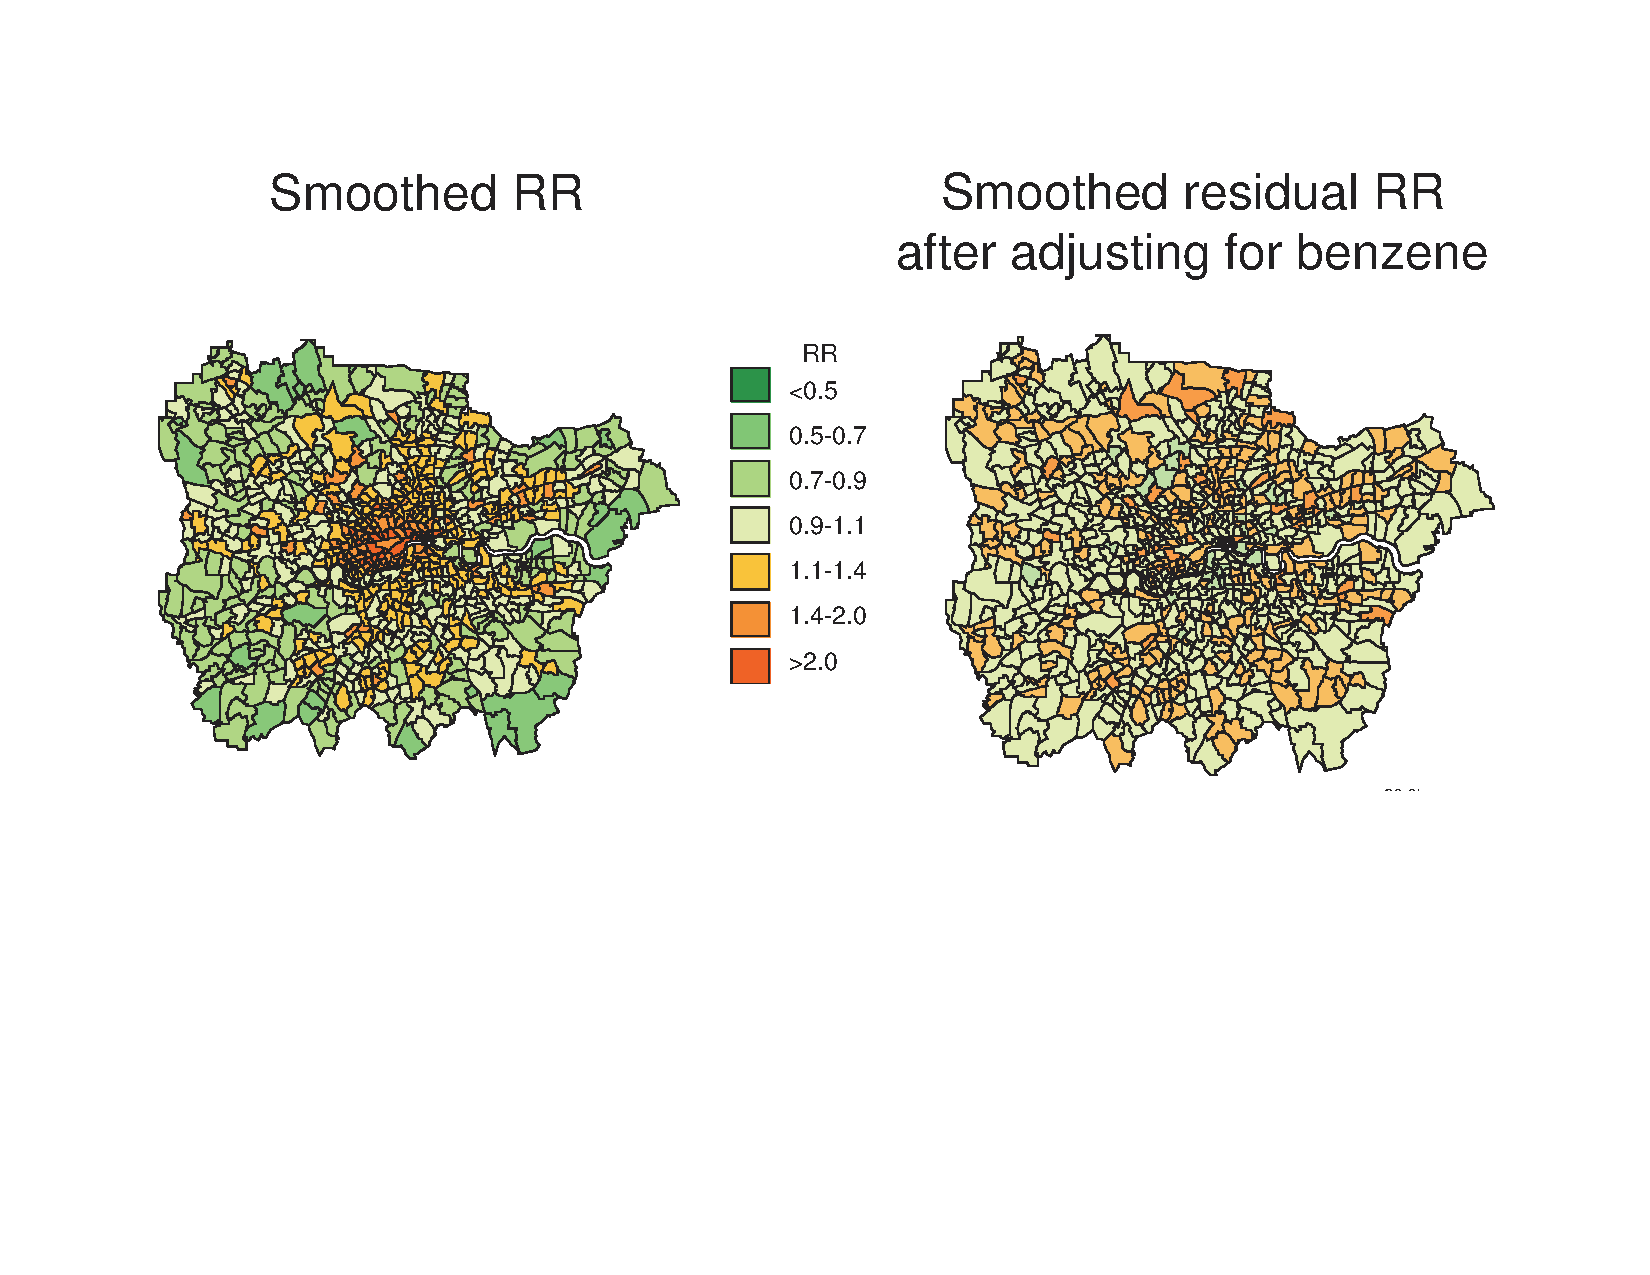
\includegraphics{figures/leuk-maps-adjrr}}}
\end{frame}

%%%%%%%%%%%%%%%%%%%%%%%%%%%%%%%%%%%%%%%%%%%%%%%%%%%%%%%%%%%%%

\begin{frame}
    \frametitle{Longitudinal data}
    \begin{itemize}
        \item Arise in studies where individual (or units) are measured repeatedly over time\vspace{2mm}
        \item For a given individual, observations over time will be typically dependent\vspace{2mm}
        \item Longitudinal data can arise in various forms:\vspace{1mm}
        \begin{itemize}
            \item continuous or discrete response\\- discrete response can be binary/binomial, categorical or counts\vspace{1mm}
            \item equally spaced or irregularly spaced\vspace{1mm}
            \item same or different time points for each individual\vspace{1mm}
            \item with or without missing data\vspace{1mm}
            \item many or few time points, $T$\vspace{1mm}
            \item many or few individuals or units, $n$
        \end{itemize}
    \end{itemize}
\end{frame}

\begin{frame}
    \frametitle{Analysing longitudinal data}
    \begin{itemize}
        \item There are many different ways to analyse longitudinal data\vspace{2mm}
%        \item This is a very big field, so we have to be selective\vspace{2mm}
        \item The key feature of longitudinal data is the need to account for the dependence structure of the data\vspace{2mm}
        \item Two common methods:\vspace{1mm}
        \begin{itemize}
            \item random effects (hierarchical) models\vspace{1mm}
            \item autoregressive models\vspace{2mm}
        \end{itemize}
        \item Here, we will focus on random effects models
    \end{itemize}
\end{frame}

\begin{frame}
    \frametitle{HAMD Example: antidepressant clinical trial}
    \begin{itemize}
       \item 6 centre clinical trial, comparing 3 treatments of depression\vspace{2mm}
       \item 367 subjects randomised to one of 3 treatments\vspace{2mm}
       \item Subjects rated on Hamilton depression score (HAMD) on 5 weekly visits\vspace{1mm}
       \begin{itemize}
            \item week 0 before treatment\vspace{1mm}
            \item weeks 1-4 during treatment\vspace{2mm}
       \end{itemize}
       \item HAMD score takes values 0-50\vspace{1mm}
       \begin{itemize}
            \item the higher the score, the more severe the depression\vspace{2mm}
       \end{itemize}
       \item Subjects drop out from week 2 onwards, but for now we\vspace{1mm}
       \begin{itemize}
            \item ignore the subjects who dropped out\vspace{1mm}
            \item analyse the 246 complete cases\vspace{2mm}
       \end{itemize}
       \item Data was previously analysed by Diggle and Kenward (1994)
    \end{itemize}
\end{frame}

\begin{frame}
    \frametitle{HAMD Example: data}
    \begin{center}
        \scalebox{0.75}{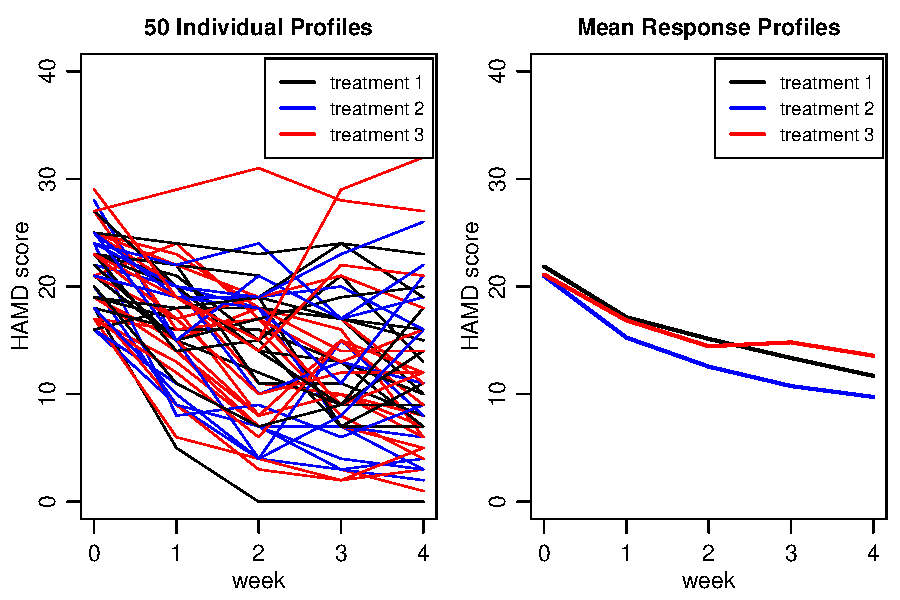
\includegraphics{figures/ccprofiles.pdf}}
    \end{center}
\end{frame}

\begin{frame}
    \frametitle{HAMD Example: objective}
    \begin{itemize}
        \item Study objective: are there any differences in the effects of the 3 treatments on the change in HAMD score over time?\vspace{2mm}
        \item The variables we will use are:\vspace{1mm}
        \begin{itemize}
            \item[y:] Hamilton depression (HAMD) score\vspace{1mm}
            \item[t:] treatment\vspace{1mm}
            \item[w:] week\vspace{2mm}
        \end{itemize}
        \item For simplicity we will\vspace{1mm}
        \begin{itemize}
            \item ignore any centre effects\vspace{1mm}
            \item assume linear relationships\vspace{2mm}
        \end{itemize}
        \item The models we will consider are:\vspace{1mm}
        \begin{itemize}
            \item a non-hierarchical model (standard linear regression)\vspace{1mm}
            \item a hierarchical model with random intercepts\vspace{1mm}
           \item a hierarchical model with random intercepts and random slopes\vspace{1mm}
        \end{itemize}
    \end{itemize}
\end{frame}

\begin{frame}
    \frametitle{\large{HAMD Example: a Bayesian (non-hierarchical) linear model (LM)}}
    \begin{itemize}
        \item Specification:\vspace{2mm}
        \begin{itemize}
            \item probability distribution for responses:\vspace{0mm}
                $$y_{iw} \sim \mbox{Normal}(\mu_{iw},\sigma^2)$$\vspace{-4mm}
            \begin{itemize}
                \item[$y_{iw}$ =] the HAMD score for individual $i$ in week $w$ (weeks 0,\ldots,4)\vspace{2mm}
            \end{itemize}
            \item linear predictor:
                $\mu_{iw}=\alpha+\beta_{treat(i)}w$\vspace{2mm}
            \begin{itemize}
                \item[$treat(i)$ =] the treatment indicator of individual $i$, so it can take values 1, 2 or 3\vspace{1mm}
                \item[$w$ =] the week of the visit, takes value 0 for visit before treatment and values 1-4 for follow-up visits\vspace{2mm}
            \end{itemize}
        \end{itemize}
        \item In this model no account is taken of the repeated structure (observations are nested within individuals)\vspace{2mm}
        \item Assume vague priors for all parameters:
            \begin{eqnarray*}
                \alpha, \beta_1, \beta_2, \beta_3  & \sim & \mbox{Normal}(0,10000) \\[2pt]
                \frac{1}{\sigma^2} & \sim & \mbox{Gamma}(0.001,0.001)
            \end{eqnarray*}
    \end{itemize}
\end{frame}

\begin{frame}
    \frametitle{HAMD Example: a Bayesian hierarchical linear model}
    \begin{itemize}
    \item Modify LM to allow a separate intercept for each individual:
    \small
    \begin{eqnarray*}
        y_{iw} & \sim & \mbox{Normal}(\mu_{iw},\sigma^2) \\
        \mu_{iw}  & = & \textcolor{red}{\alpha_i}+\beta_{treat(i)}w
    \end{eqnarray*}
    \normalsize
%    We are assuming that \textit{conditionally} on $\alpha_i$, $\{y_{iw}, w=0,\ldots,4 \}$ are independent\vspace{1mm}
    \item Assume that all the $\{\alpha_i\}$ follow a \textit{common} prior distribution, e.g.
    \small \textcolor{red}{$$\alpha_i \sim \mbox{Normal}(\mu_{\alpha}, \sigma^2_{\alpha}) \;\;\;\; i=1,\ldots,246$$} \normalsize\vspace{-5mm}
    \item[] Here we are assuming exchangeability between all the individuals\vspace{1mm}
    \item We may then assume vague priors for the \textit{hyperparameters} of the population distribution:
    \textcolor{red}{\small
    \begin{eqnarray*}
        \mu_{\alpha} & \sim & \mbox{Normal}(0,10000) \\
        \sigma_{\alpha} & \sim & \mbox{Uniform}(0,100)
    \end{eqnarray*}}
    \normalsize
    \vspace{-12pt}
    \item This is an example of a \textit{Hierarchical LM} or \textit{Linear Mixed Model (LMM)} or \textit{Random Intercepts} model
    \end{itemize}
\end{frame}

\begin{frame}[label=current]
    \frametitle{HAMD Example: DAGs for LM and LMM}
    \centerline{\scalebox{0.8}{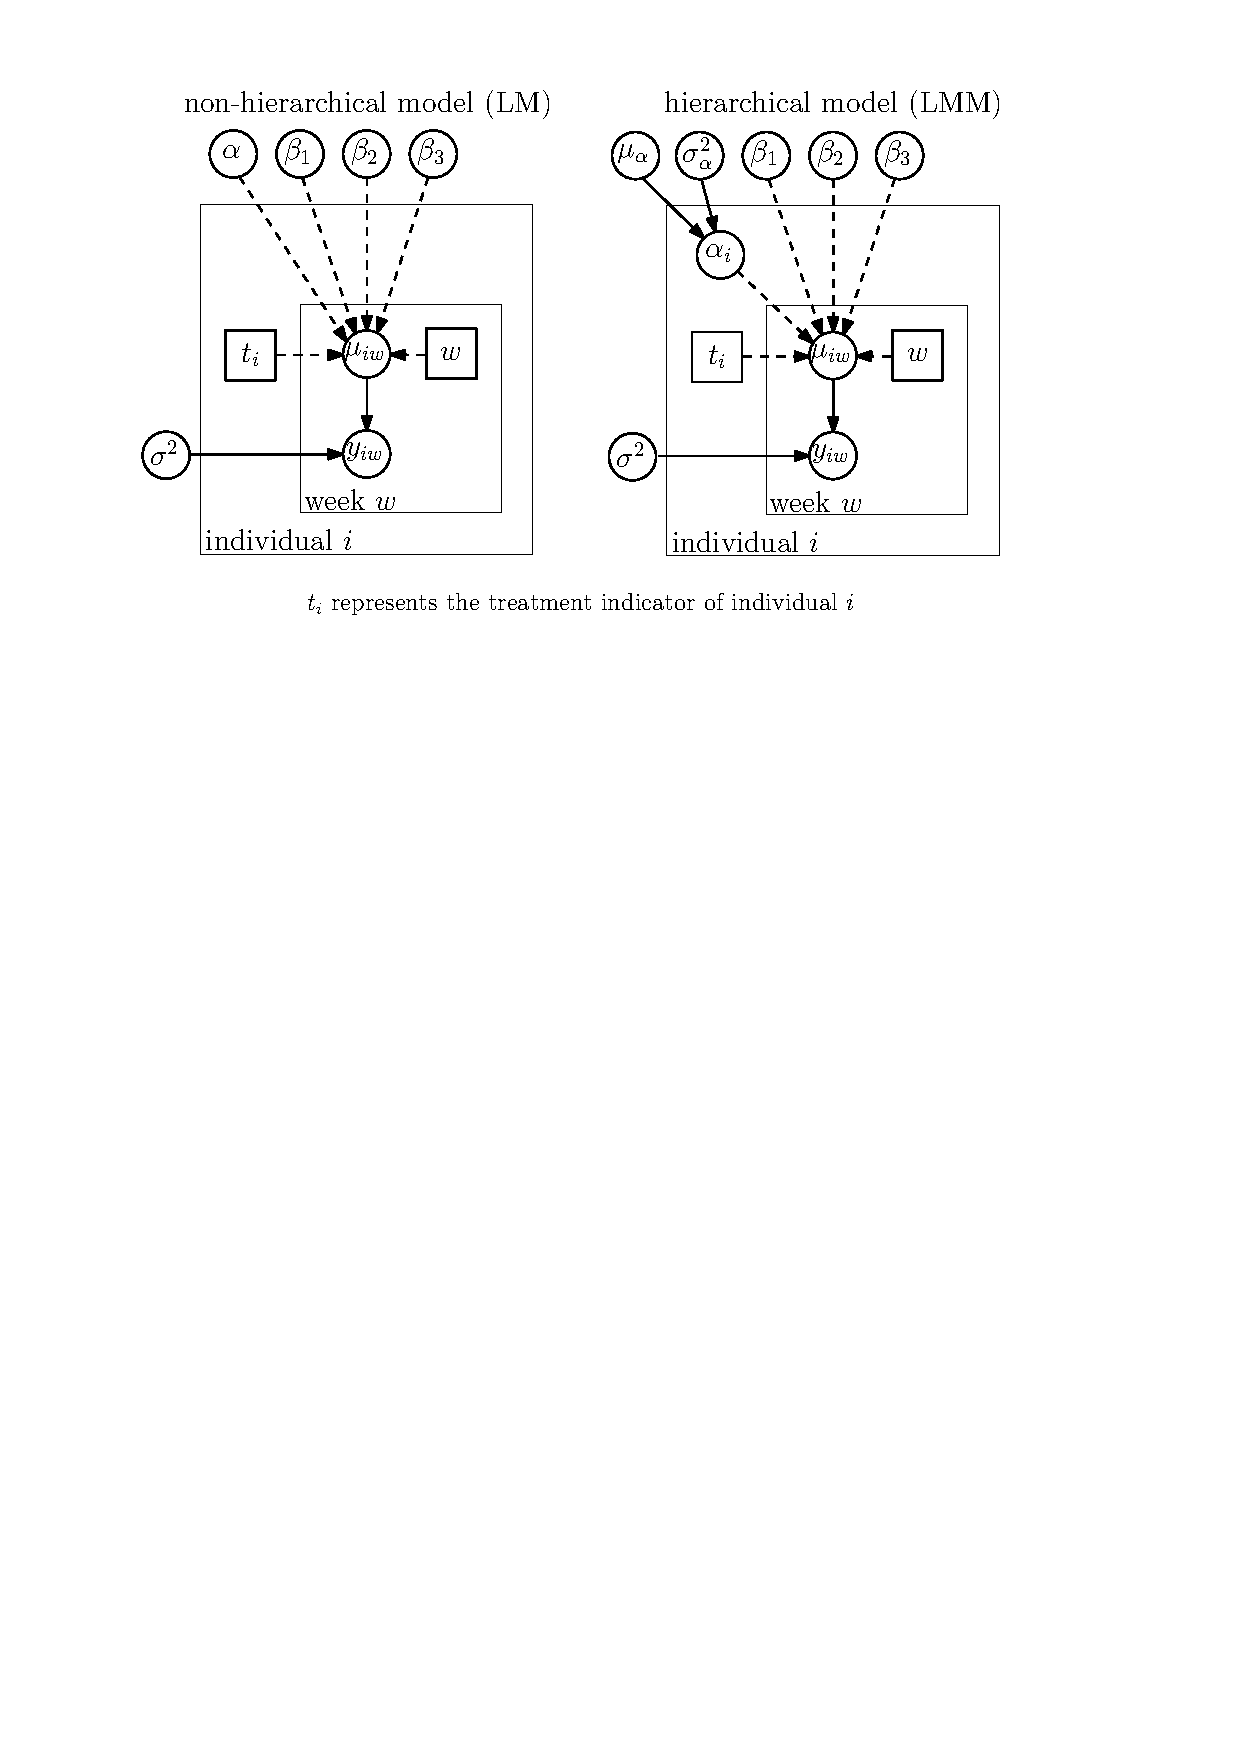
\includegraphics{figures/HAMDdags.pdf}}}
\end{frame}

\begin{frame}[containsverbatim]
    \frametitle{HAMD Example: WinBUGS code for LM and LMM}
    \vspace{2mm} Part of WinBUGS code for non-hierarchical model:
    \footnotesize
    \begin{ColorVerbatim}			
  for (i in 1:N) \{ # N individuals
    for (w in 1:W) \{ # W weeks			
      hamd[i,w]~dnorm(mu[i,w],tau)
      mu[i,w]<-\color{red}{alpha}\color{black}{+beta[treat[i]]*(w-1)}
    \}					
  \}
  # specification of priors ....			
    \end{ColorVerbatim}
    \vspace{1mm} \normalsize Part of WinBUGS code for hierarchical model:
    \footnotesize
    \begin{ColorVerbatim}
  for (i in 1:N) \{ # N individuals
    for (w in 1:W) \{ # W weeks			
      hamd[i,w]~dnorm(mu[i,w],tau)
      mu[i,w]<-\color{red}{alpha[i]}\color{black}{+beta[treat[i]]*(w-1)}
    \}
    \color{red}{alpha[i]~dnorm(alpha.mu,alpha.tau) # random intercepts}					
  \}
  # specification of priors ....	
    \end{ColorVerbatim}
\end{frame}

\begin{frame}[containsverbatim]
    \frametitle{HAMD Example: WinBUGS code for priors}
    \vspace{2mm} Prior specification for non-hierarchical model:
    \footnotesize
    \begin{ColorVerbatim}
\color{red}{alpha~dnorm(0,0.00001)}		
for (t in 1:T)\{  # T treatments	
  beta[t]~dnorm(0,0.00001)
  \}						
tau~dgamma(0.001,0.001)
sigma.sq<-1/tau  # Normal errors		
    \end{ColorVerbatim}
    \vspace{1mm} \normalsize Prior specification for hierarchical model:
    \footnotesize
    \begin{ColorVerbatim}
\color{red}{alpha.mu~dnorm(0,0.00001)}
\color{red}{alpha.sigma~dunif(0,100) }
\color{red}{alpha.sigma.sq<-pow(alpha.sigma,2)}
\color{red}{alpha.tau<-1/alpha.sigma.sq}
for (t in 1:T)\{  # T treatments	
  beta[t]~dnorm(0,0.00001)
  \}								
tau~dgamma(0.001,0.001)
sigma.sq<-1/tau  # Normal errors	
    \end{ColorVerbatim}
\end{frame}

\begin{frame}
    \frametitle{HAMD Example: LM and LMM fitted lines}
    \vspace{-2mm}
    \begin{center}
        \scalebox{0.65}{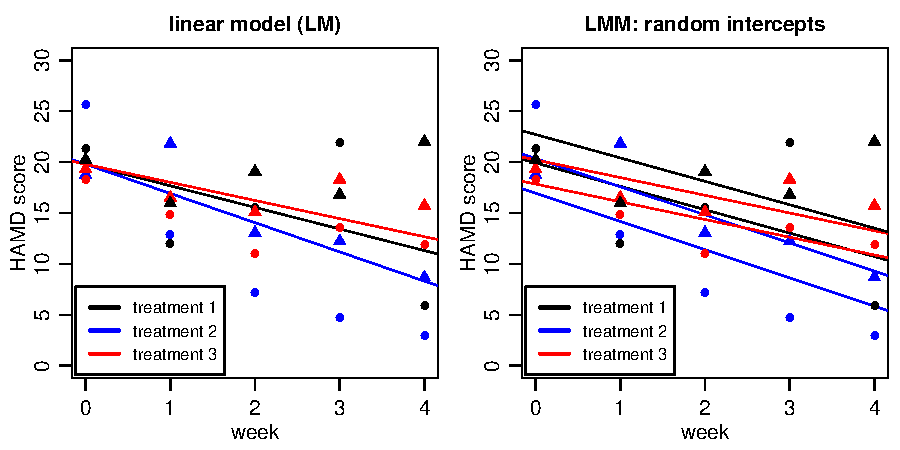
\includegraphics{figures/lineplot1.pdf}}\\\vspace{-2mm}
        \footnotesize circles and triangles represent scores for 6 individuals (2 for each treatment) \normalsize
    \end{center}
    \begin{itemize}\vspace{-2mm}\small
        \item LM:
        \begin{itemize}
            \item 3 regressions lines fitted, 1 for each treatment
            \item each treatment has the same intercept, but a different slope
        \end{itemize}\vspace{1mm}
        \item LMM:
        \begin{itemize}
            \item each individual has a different regression line
            \item but for each treatment, individuals have the same slope
        \end{itemize}
    \end{itemize}
    \normalsize
\end{frame}

\begin{frame}
    \frametitle{HAMD Example: results for LM and LMM}
    \vspace{-5mm}
    \renewcommand{\arraystretch}{1.3}
    \input{tables/LMvLMM}
    \renewcommand{\arraystretch}{1}
    Note
    \begin{itemize}
        \item the variability in the intercept in the hierarchical model
        \item how the residual variance ($\sigma^2$) is reduced when random effects are incorporated
    \end{itemize}
    \vspace{-2mm}
\end{frame}

\begin{frame}
    \frametitle{HAMD Example: revisiting the data}
    \vspace{-10mm}
    \begin{columns}
        \begin{column}{5cm}
            \begin{center}
                \scalebox{0.75}{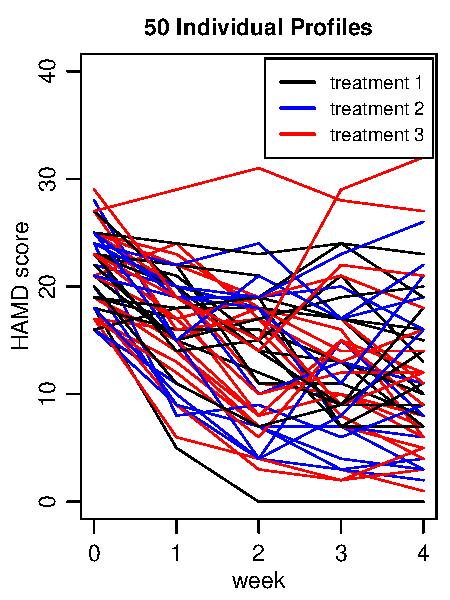
\includegraphics{figures/ccindivids.pdf}}
            \end{center}
        \end{column}
        \begin{column}{5cm}
            The plot of the raw data\vspace{1mm}
            \begin{itemize}
                \item indicates that separate intercepts are appropriate\vspace{1mm}
                \item also suggests including separate slopes\vspace{2mm}
            \end{itemize}
            So we add random slopes to the hierarchical model
        \end{column}
    \end{columns}
\end{frame}

\begin{frame}[containsverbatim]
    \frametitle{HAMD Example: adding random slopes}
    \small
    \begin{itemize}
    \item Modify LMM to allow a separate slope for each individual:
    \begin{eqnarray*}
        y_{iw} & \sim & \mbox{Normal}(\mu_{iw},\sigma^2) \\
        \mu_{iw}  & = & \alpha_i+\beta_{(treat(i),\textcolor{red}{i})}w
    \end{eqnarray*}
    \item As for the $\{\alpha_i\}$, assume that the $\{\beta_{(1,i)}\}$,$\{\beta_{(2,i)}\}$ \& $\{\beta_{(3,i)}\}$ follow \textit{common} prior distributions with vague priors on their \textit{hyperparameters}
    \end{itemize}
    \scriptsize
    \begin{ColorVerbatim}
  for (i in 1:N) \{  # N individuals
    for (w in 1:W) \{  # W weeks			
      hamd[i,w]~dnorm(mu[i,w],tau)
      mu[i,w]<-alpha[i]+beta[treat[i]\color{red}{,i}\color{black}{]*(w-1)}
    \}
    alpha[i]~dnorm(alpha.mu,alpha.tau)
   \color{red}{ for (t in 1:T)\{beta[t,i]~dnorm(beta.mu[t],beta.tau[t])\}	}				
  \}
  # Priors
  for (t in 1:T)\{  # T treatments	
    \color{red}{beta.mu[t]~dnorm(0,0.00001)}
    \color{red}{beta.sigma[t]~dunif(0,100)}
    \color{red}{beta.sigma.sq[t]<-pow(beta.sigma[t],2)}
    \color{red}{beta.tau[t]<-1/beta.sigma.sq[t]}
  \}	# specification of other priors as before ....							
    \end{ColorVerbatim}
    \normalsize
\end{frame}

\begin{frame}
    \frametitle{HAMD Example: random intercepts and slopes}
    \vspace{-2mm}
    \begin{center}
        \scalebox{0.65}{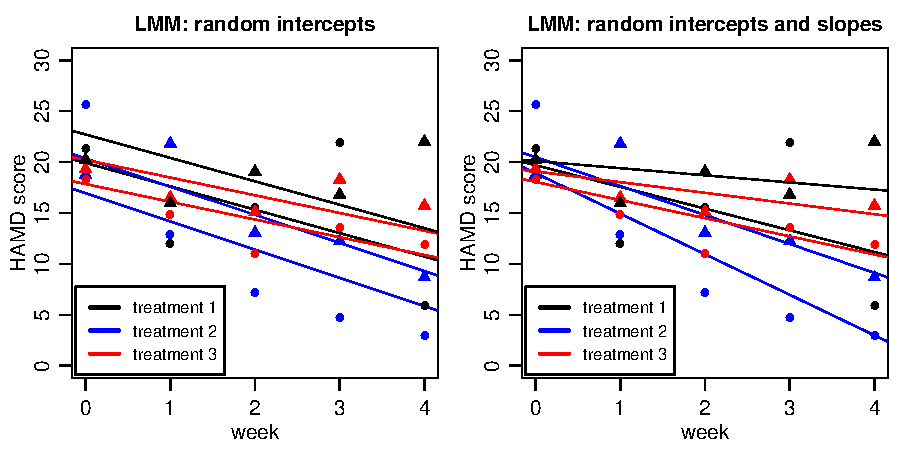
\includegraphics{figures/lineplot2.pdf}}\\\vspace{-2mm}
        \footnotesize circles and triangles represent scores for 6 individuals (2 for each treatment) \normalsize
    \end{center}
    \begin{itemize}\vspace{-2mm}\small
        \item LMM with random intercepts only:
        \begin{itemize}
            \item each individual has a different regression line
            \item but for each treatment, only intercept varies by individual
        \end{itemize}\vspace{1mm}
        \item LMM with random intercepts and random slopes:
        \begin{itemize}
            \item now intercepts and slopes both vary
            \item better fit for each individual
        \end{itemize}
    \end{itemize}
    \normalsize
\end{frame}

\begin{frame}
    \frametitle{HAMD Example: results comparison}
    \vspace{-2mm}
    \setlength{\tabcolsep}{3pt}
    \renewcommand{\arraystretch}{1.2}
    \input{tables/LMvLMM1vLMM2}
    \renewcommand{\arraystretch}{1}
    \setlength{\tabcolsep}{6pt}  % return to default
\end{frame}

\begin{frame}[containsverbatim]
    \frametitle{HAMD Example: interpretation of results}
    \begin{itemize}
        \item Study objective: are there any differences in the effects of the 3 treatments on the change in HAMD score over time?\vspace{2mm}
        \item So we are particularly interested in the differences in the slope parameters, i.e.~\vspace{1mm}
        \begin{itemize}
            \item $\beta_1-\beta_2$, $\beta_1-\beta_3$ and $\beta_2-\beta_3$ or\vspace{1mm}
            \item $\mu_{\beta_1}-\mu_{\beta_2}$, $\mu_{\beta_1}-\mu_{\beta_3}$ and $\mu_{\beta_2}-\mu_{\beta_3}$ for models with random slopes\vspace{2mm}
        \end{itemize}
        \item To monitor these contrasts, add the following lines of BUGS code
        \footnotesize
    \begin{verbatim}
# Calculate contrasts
contrasts[1]<-beta[1]-beta[2]
contrasts[2]<-beta[1]-beta[3]
contrasts[3]<-beta[2]-beta[3]		
    \end{verbatim}
    \vspace{-3mm}or
    \footnotesize
    \begin{verbatim}
contrasts[1]<-beta.mu[1]-beta.mu[2] ...
    \end{verbatim}
    \end{itemize}
\end{frame}

\begin{frame}
    \frametitle{HAMD Example: contrasts}
    \renewcommand{\arraystretch}{1.2}
    \setlength{\tabcolsep}{3pt}
    \input{tables/contrasts}
    \setlength{\tabcolsep}{6pt}  % return to default
    \renewcommand{\arraystretch}{1}
    Density plots for hierarchical 2
    \begin{center}
        \scalebox{0.4}{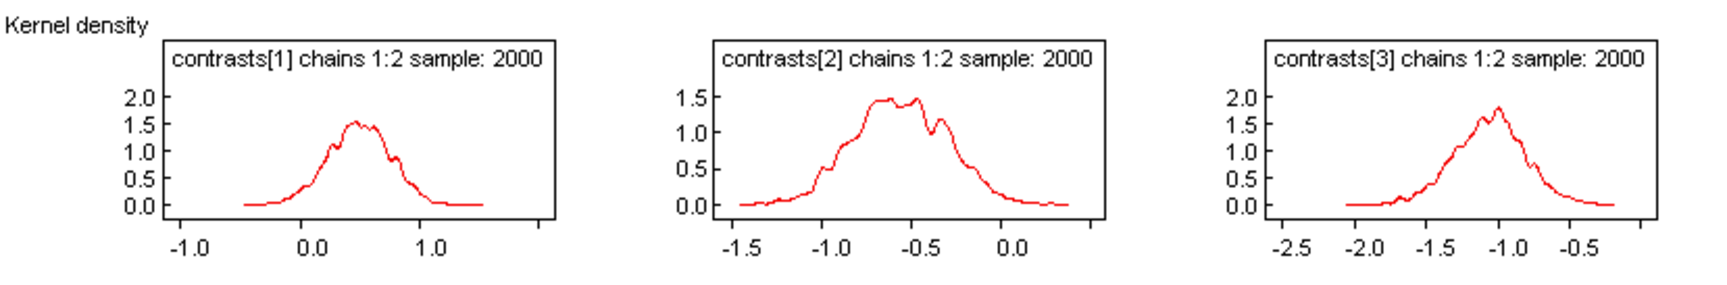
\includegraphics{figures/density.pdf}}\\
    \end{center}
\end{frame}

%%%%%%%%%%%%%%%%%%%%%%%%%%%%%%%%%%%%%%%%%%%%%%%%%%%%%%%%%%%%%

\begin{frame}
\frametitle{Cross-classified random effects models}
\bibig
\I Straightforward to extend basic hierarchical model to include
   non-nested random effects structures, e.g.\vspace{2mm}
   \bibig
   \I THM measurements cross-classified within zones and years\vspace{1mm}
   \I pupils cross-classified within primary and secondary schools\vspace{2mm}
   \eibig
\I Easiest to formulate cross-classified models in BUGS using nested index notation
  (see example)
\eibig
\end{frame}

\begin{frame}[fragile]
\frametitle{Example: Schools -- exam scores cross-classified by primary and secondary school}
\bibig
\I These data were obtained from the MLwiN website \\
   \verb+www.mlwin.com/softrev/2lev-xc.html+\vspace{1mm}
\I We use a random sample of 800 children who attended 132 primary schools and 19 secondary schools in Scotland\vspace{1mm}
\I The following variables were used\vspace{0.5mm}
\begin{itemize}
\I[{\tt Y}] exam attainment score of pupils at age 16\vspace{0.5mm}
\I[{\tt VRQ}] verbal reasoning score taken on secondary school entry\vspace{0.5mm}
\I[{\tt SEX}] pupil's gender (0 = boy, 1 = girl)\vspace{0.5mm}
\I[{\tt PID}] primary school identifying code\vspace{0.5mm}
\I[{\tt SID}] secondary school identifying code\vspace{1mm}
\end{itemize}
\I {\bf Model 1:} Normal hierarchical model with independent random effects
   for primary school and secondary school\vspace{1mm}
\I {\bf Model 2:} Verbal reasoning score + gender included as \lq fixed' covariate effects
   (but note that in Bayesian framework, \lq fixed' effect coefficients are
   still assigned prior distributions)
\eibig
\end{frame}

\begin{frame}[fragile]
\frametitle{BUGS model code (Model 2)}
\vspace{-0.3cm}
\begin{footnotesize}
\begin{ColorVerbatim}
for(i in 1:Nobs) \{
 Y[i] ~ dnorm(mu[i], tau.e)
 mu[i] <- alpha + beta[1]*SEX[i] + beta[2]*VRQ[i] +
                \color{red}{theta.ps[PID[i]]}\color{black}{ +}\color{blue}{ theta.ss[SID[i]]}
\}
### random effects distributions
\color{red}{ for(j in 1:Nprim) \{ theta.ps[j] ~ dnorm(0, tau.ps) \} # primary}
\color{blue}{ for(k in 1:Nsec) \{ theta.ss[k] ~ dnorm(0, tau.ss) \} # secondary}
### priors on regression coefficients and variances
 tau.e ~ dgamma(0.001, 0.001)
 sigma2.e <- 1/tau.e           # residual error variance
\color{red}{ tau.ps ~ dgamma(0.001, 0.001)}
\color{red}{ sigma2.ps <- 1/tau.ps         # between primary school var.}
\color{blue}{ tau.ss ~ dgamma(0.001, 0.001)}
\color{blue}{ sigma2.ss <- 1/tau.ss         # between secondary school var.}
 alpha ~ dnorm(0, 0.000001)    # intercept
 for(q in 1:2) \{beta[q] ~ dnorm(0, 0.000001)\} # regression coeff.
### percentage of total variance explained
\color{red}{ VPC.ps <- sigma2.ps/(sigma2.e+sigma2.ps+sigma2.ss) # primary}
\color{blue}{ VPC.ss <- sigma2.ss/(sigma2.e+sigma2.ps+sigma2.ss) # secondary}
\end{ColorVerbatim}
\end{footnotesize}
\end{frame}

\begin{frame}
\frametitle{Results}
\renewcommand{\arraystretch}{1.2}
\begin{center}
\begin{tabular}{l  c  c c c }
\hline
Parameters & \multicolumn{2}{c}{Model 1}  & \multicolumn{2}{c}{Model 2}  \\
\hline
$\alpha$ &  5.53 & (5.17, 5.88) & 5.85 & (5.59, 6.10)   \\
$\beta_1$ (sex) & -- & --  &  0.23 & (-0.08, 0.53) \\
$\beta_2$ (VRQ) & -- & -- & 0.16 & (0.15, 0.17) \\
$\sigma_{[e]}^2$ & 8.18 & (7.35, 9.10)&  4.49 & (4.03, 5.00) \\
$\sigma_{[ps]}^2$& 1.12 & (0.43, 1.98) & 0.36 & (0.08, 0.70) \\
$\sigma_{[ss]}^2$& 0.19 & (0.10, 0.82) & 0.02 & (0.0007, 0.12)\\
VPC$_{ps}$ & 11.8\%  & (4.7\%, 19.8\%) & 7.4\% & (1.5\%, 13.8\%) \\
VPC$_{ss}$ & 2.0\% &  (0.1\%, 8.3\%) & 0.4\% & (0.01\%, 2.4\%) \\
\hline
DIC & 4008 & &  3514 & \\
$p_D$ & 58.0 & & 43.8 & \\
\hline
\end{tabular}
\end{center}
\renewcommand{\arraystretch}{1}
\end{frame}

\begin{frame}
\begin{center}
\scalebox{0.42}{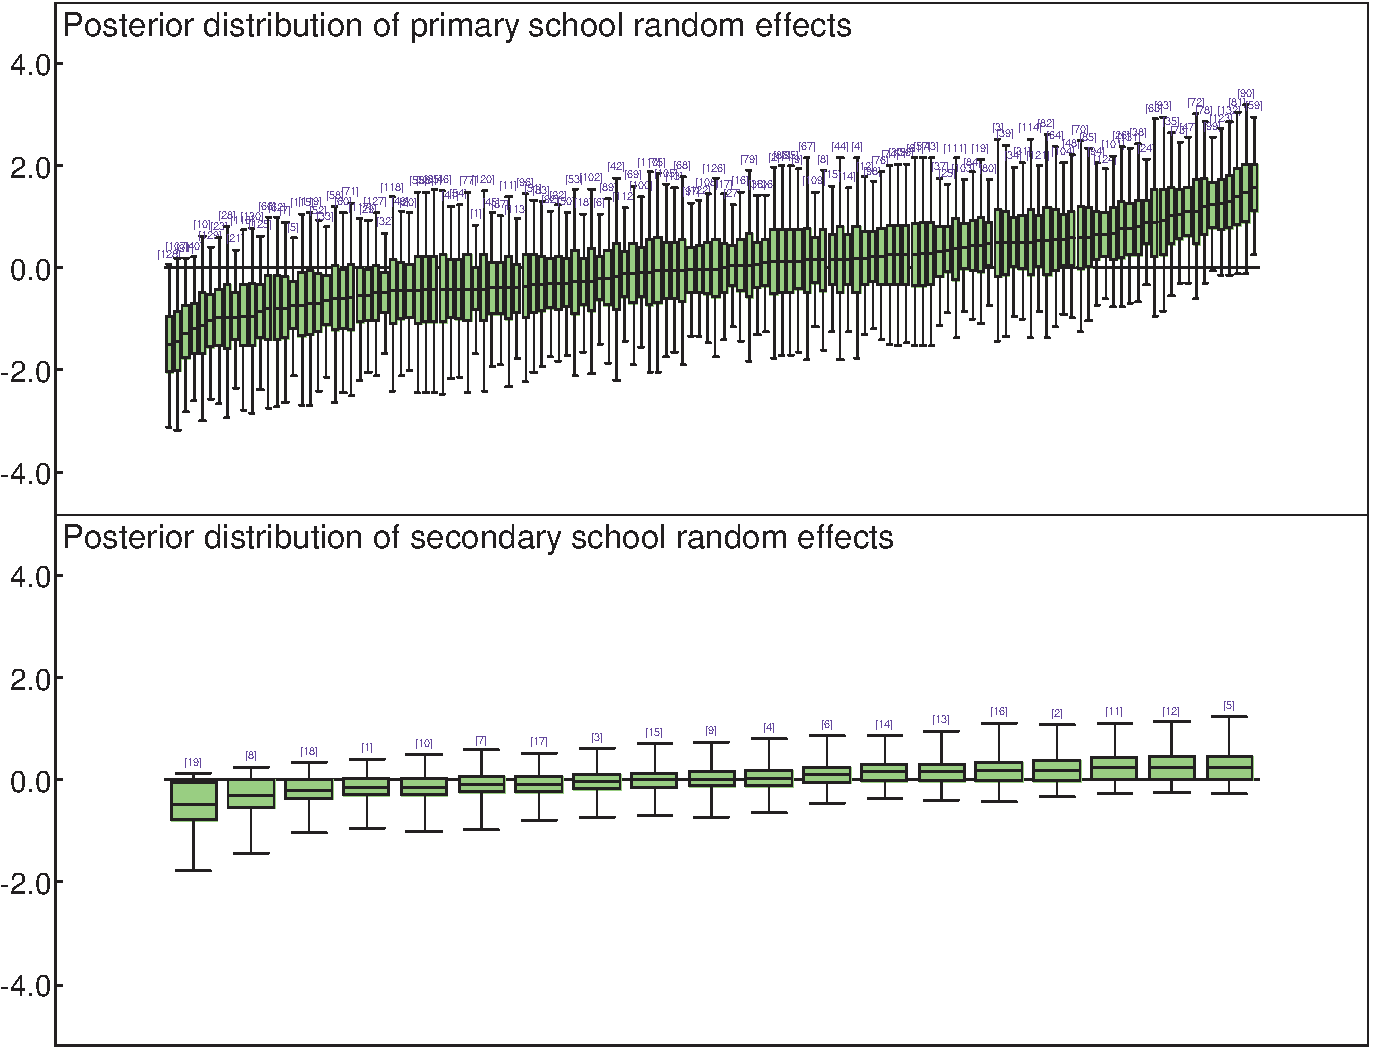
\includegraphics{figures/xc-boxplots.pdf}}
\end{center}
\end{frame}

\begin{frame}
    \frametitle{In conclusion}
    Bayesian analysis is useful because it\vspace{2mm}
    \begin{itemize}
        \item More closely approximates our natural thought processes\vspace{2mm}
        \item Allows relevant questions to be addressed\vspace{2mm}
        \item Uses all available evidence efficiently\vspace{2mm}
        \item Is powerful and extremely flexible, allowing realistic models to be fitted to complex data sets in a coherent framework\vspace{2mm}
    \end{itemize}
    \pause
    This course was an introduction to equip you with the basic tools, but you have only just begun to explore the possibilities\vspace{4mm}
    \pause
    \centerline{\alert{Building Bayesian models can be challenging, but fun!}}
\end{frame}

\end{document}